\documentclass[12pt]{article}

\usepackage{graphicx}
\usepackage[a4paper,margin=1in]{geometry}
\usepackage{amsmath,amssymb}
\usepackage{textcomp}

\begin{document}

\noindent
\begin{minipage}{0.38\textwidth}
\begin{flushleft}
\textbf{KUNE PAVITHRA}\\[0.2cm]
\textbf{COMET FWC 69}
\end{flushleft}
\end{minipage}
\begin{minipage}{0.6\textwidth}
\begin{flushright}

\includegraphics[width=0.75\textwidth]{IIITB_logo_with_Institute_Name_jpeg1.jpg}
\end{flushright}
\end{minipage}

\vspace{0.5cm}

\begin{center}
{\fontsize{24}{28}\selectfont
\textbf{Mathematics Olympiad Task (Q14--Q26)}
}
\end{center}

\section*{Q14}

In Fig. 6, find the area of the shaded region enclosed between two concentric circles of radii 7 cm and 14 cm where $\angle AOC = 40^\circ$. (Use $\pi = \tfrac{22}{7}$)

\begin{center}
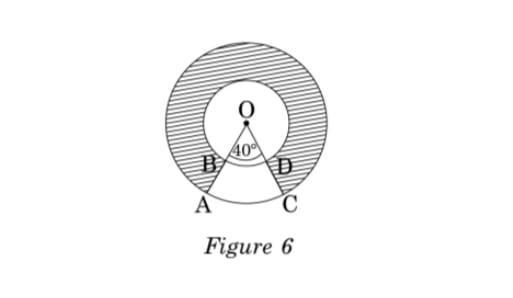
\includegraphics[width=0.5\textwidth]{figure6.jpg}
\end{center}

\section*{Q15}

If the ratio of the sum of first $n$ terms of two A.P.'s is $(7n+1):(4n+27)$, find the ratio of their $m$th terms.

\section*{Q16}

Solve for $x$:

\[
\frac{1}{(x-1)(x-2)} + \frac{1}{(x-2)(x-3)} = \frac{2}{3},
\quad x \neq 1,2,3
\]

\section*{Q17}

A conical vessel, with base radius 5 cm and height 24 cm, is full of water. This water is emptied into a cylindrical vessel of base radius 10 cm. Find the height to which the water will rise in the cylindrical vessel. (Use $\pi = \tfrac{22}{7}$)

\section*{Q18}

A sphere of diameter 12 cm is dropped in a right circular cylindrical vessel partly filled with water. If the sphere is completely submerged in water, the water level in the cylindrical vessel rises by 32 cm. Find the diameter of the cylindrical vessel.

\section*{Q19}

A man standing on the deck of a ship, which is 10 m above water level, observes the angle of elevation of the top of a hill as $60^\circ$ and the angle of depression of the base of the hill as $30^\circ$. Find the distance of the hill from the ship and the height of the hill.

\section*{Q20}

Three different coins are tossed together. Find the probability of getting:

(i) exactly two heads

(ii) at least two heads

(iii) at least two tails.

\section*{Q21}

Due to heavy floods in a state, thousands were rendered homeless. Fifty schools collectively offered to the state government to provide place and canvas for 1500 tents.

Each tent has a cylindrical base (radius 2.8 m, height 3.5 m) and a conical top (radius 2.8 m, height 2.1 m).

If canvas costs Rs120 per sq.m, find the amount shared by each school.

What value is generated by the problem?

(Use $\pi = \tfrac{22}{7}$)

\section*{Q22}

Prove that the lengths of the tangents drawn from an external point to a circle are equal.

\section*{Q23}

Draw a circle of radius 4 cm. Draw two tangents to the circle inclined at an angle of $60^\circ$ to each other.

\section*{Q24}

In Fig. 7, two equal circles, with centres $O$ and $O'$, touch each other at $X$.

$OO'$ produced meets the circle with centre $O'$ at $A$.

$AC$ is tangent to the circle with centre $O$, at the point $C$.

$O'D \perp AC$.

Find the value of $\tfrac{CO}{DO'}$.

\begin{center}
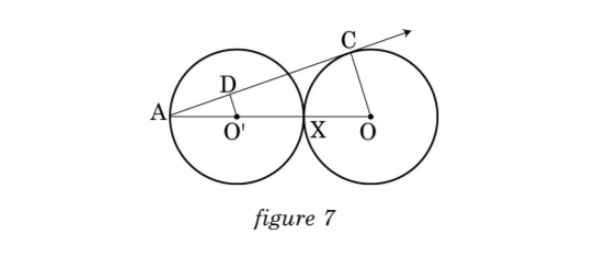
\includegraphics[width=0.5\textwidth]{figure7.jpg}
\end{center}

\section*{Q25}

Solve for $x$:

\[
\frac{1}{x+1} + \frac{1}{x+2} + \frac{1}{x+4} = \frac{2}{x},
\quad x \neq -1,-2,-4
\]

\section*{Q26}

The angle of elevation of the top $Q$ of a vertical tower $PQ$ from a point $X$ on the ground is $60^\circ$.

From a point $Y$, 40 m vertically above $X$, the angle of elevation of the top $Q$ of the tower is $45^\circ$.

Find the height of the tower $PQ$ and the distance $PX$.

(Use $\sqrt{3} = 1.73$)

\end{document}

